
% ---
% Arquivo com a metodologia do Trabalho de Conclusão de Curso do aluno
% Daniel Noriaki Kurosawa
% da Escola Politécnica da Universidade de São Paulo
% ---
	% ---
	\chapter{Metodologia}\label{cap-metodologia}
	% ---
	
	Este capítulo apresenta o método de trabalho adotado para a execução das atividades
	do projeto e divide-se em três partes: organização de tarefas, escolha de hardware e software utilizados.
	
	

	
	% ---
	\section{Planejamento}\label{sec-planejamento}
	% ---
	Inicialmente, foi elaborado um diagrama de Gantt do sistema contendo as principais etapas do projeto (\autoref{fig_gantt}) a partir do qual foram identificadas as tarefas a serem realizadas durante o projeto, que foram posteriormente transferidas para o Trello.
	\begin{figure}[h!]
	\caption{\label{fig_gantt} Diagrama de Gantt do sistema }
		\begin{center}
	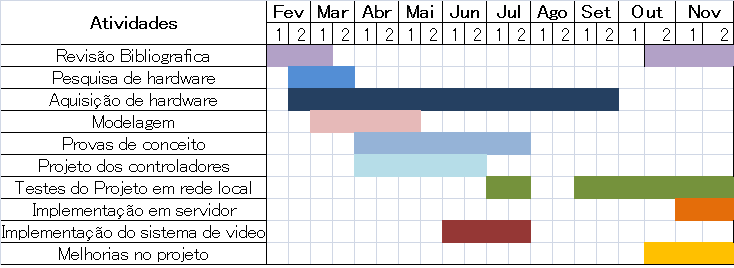
\includegraphics[width=\textwidth]{gantt.png}	
\end{center}
	\legend{Fonte: Autor}
\end{figure}

	% ---
	\subsection{Trello}\label{subsec-eap}
	% ---
	Trello é uma ferramenta de organização de projetos  baseada nos quadros Kanban da metodologia ágil. Extremamente versátil, permite uma análise rápida da situação do projeto, das etapas cumpridas e do cronograma geral do projeto. No Trello, é possível criar “boards” que agrupam listas (“lists”) de tarefas que devem ser feitas. Cada tarefa é então representada por um “card”, criado dentro de uma “list”. As “lists” criadas dentro da “board” do projeto são:\par
	
	\subparagraph{Backlog}: Tarefas que ainda precisam ser analisadas e aprovadas para serem colocadas na fase de atividades.
	\subparagraph{Sprint}: Tarefas a serem realizadas após a conclusão das tarefas sendo trabalhadas atualmente.
	\subparagraph{Doing}: Tarefas em execução.
	\subparagraph{To be verified}: Tarefas executadas a serem revisadas.
	\subparagraph{Done}: Tarefas terminadas.
	\subparagraph{Halt}: Tarefas suspensas/canceladas.

		\begin{figure}[h!]
		\caption{\label{fig_trello} Kanban do projeto usando Trello }
		\begin{center}
	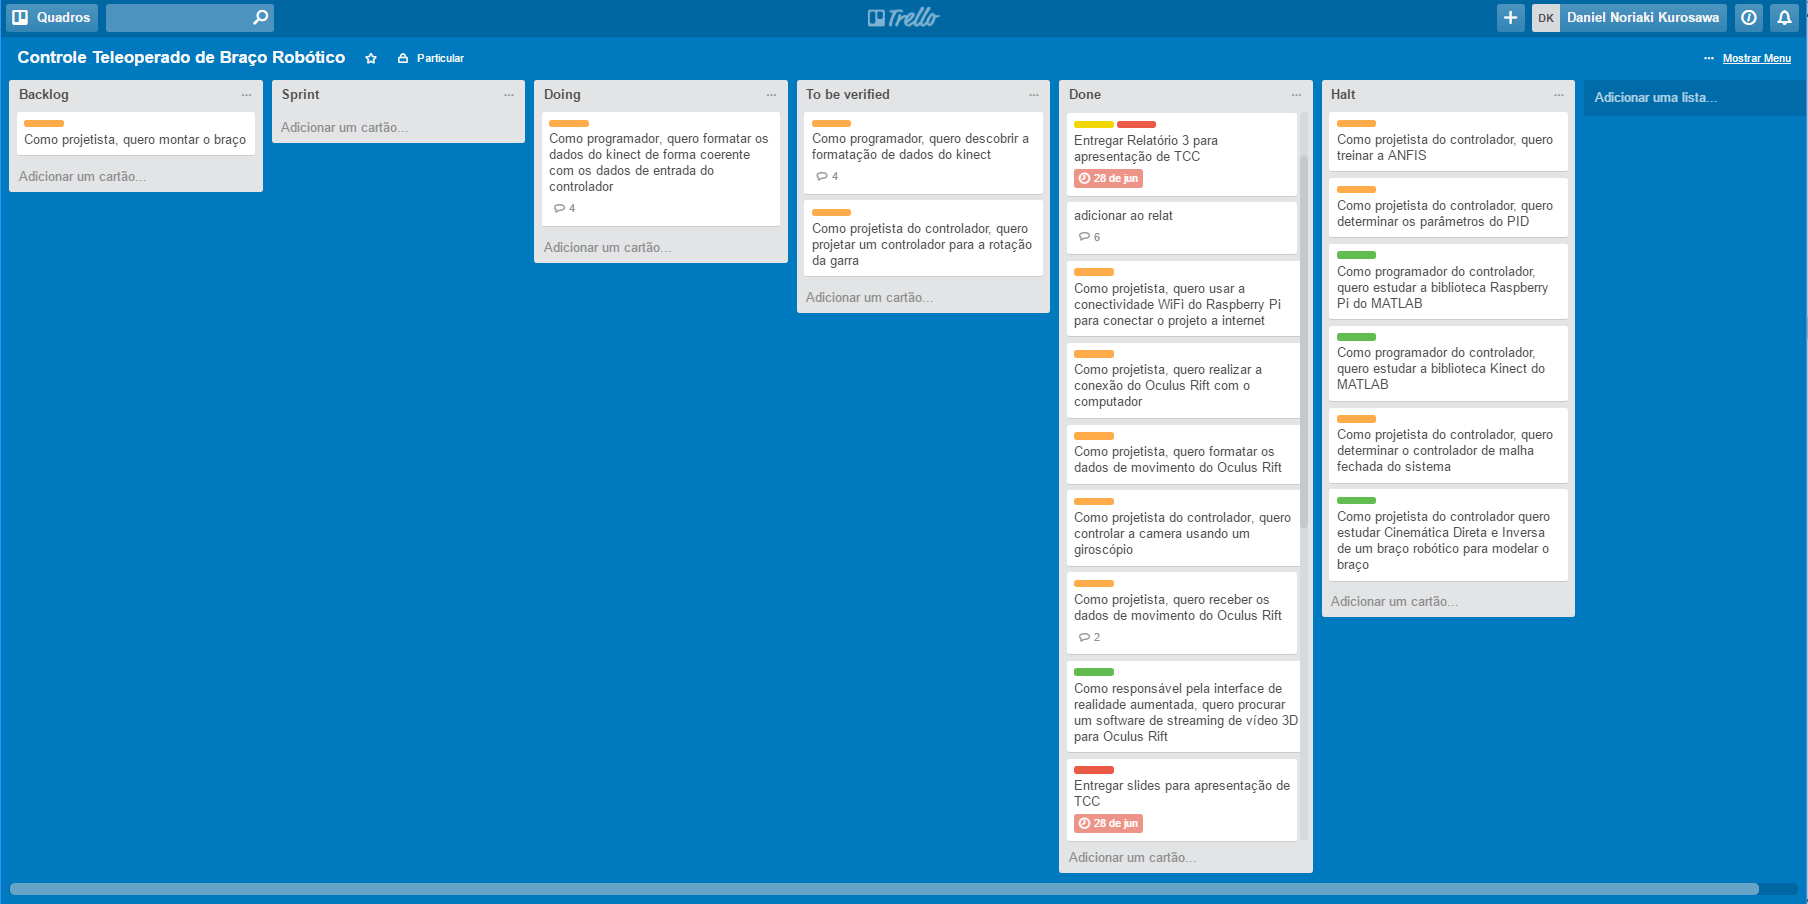
\includegraphics[width=\textwidth]{trello.png}	
	\end{center}
	\legend{Fonte: Autor}
	\end{figure}
	
	
	% ---
	\section{Programas e IDEs}\label{sec-requisitos}
	% ---
	Esta seção apresenta os principais programas e IDEs (Integrated Development Environment) utilizados durante o desenvolvimento de cada componente do sistema proposto.
		\subsection{Visual Studio 2015}\label{subsec-VSIDE}
		A aplicação para Kinect foi feita usando-se o programa Visual Studio 2015.\par
		O Visual Studio é a IDE usada pelo Kinect SDK da Microsoft para o desenvolvimento de aplicações Kinect, e permite elaborar o aplicativo e facilmente verificar os seus erros. É também a 
		Possui inúmeros exemplos de código de aplicações em C\#, C++ e Visual Basic que também auxiliam no desenvolvimento de uma aplicação.
		\begin{figure}[h!]
		\caption{\label{fig_VSIDE} Visual Studio 2015 IDE }
		\begin{center}
			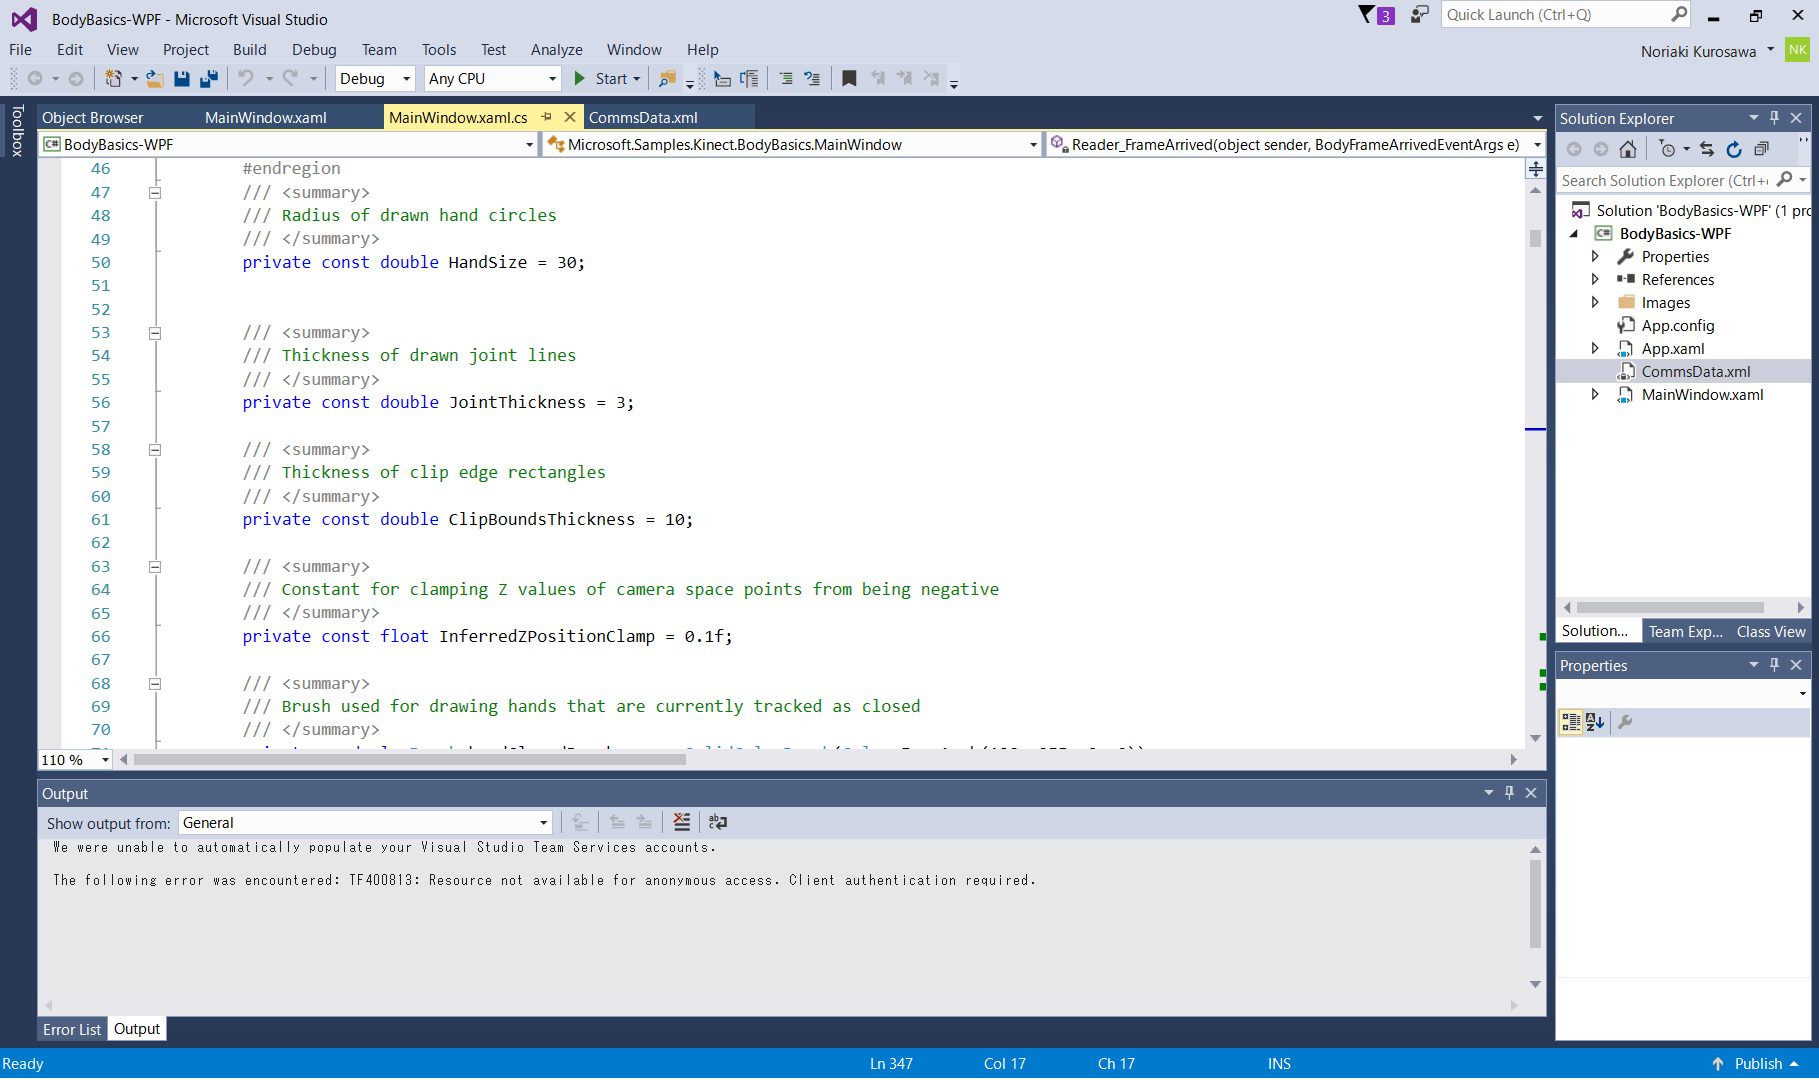
\includegraphics[width=\textwidth]{VSIDE.png}	
		\end{center}
		\legend{Fonte: Autor}
		\end{figure}
	
	
		\subsection{Raspberry Pi}\label{subsec-raspIDE}
			A configuração do servidor HTTP Apache foi escrita utilizando-se o editor de texto GNU NANO, que já vem pré-instalado no Raspberry Pi. A escolha se deu pela simplicidade da estrutura do arquivo de configuração, que não demandava grandes funcionalidades.
			\begin{figure}[h!]
		\caption{\label{fig_raspIDE} Editor de texto GNU NANO do Raspberry Pi }
		\begin{center}
			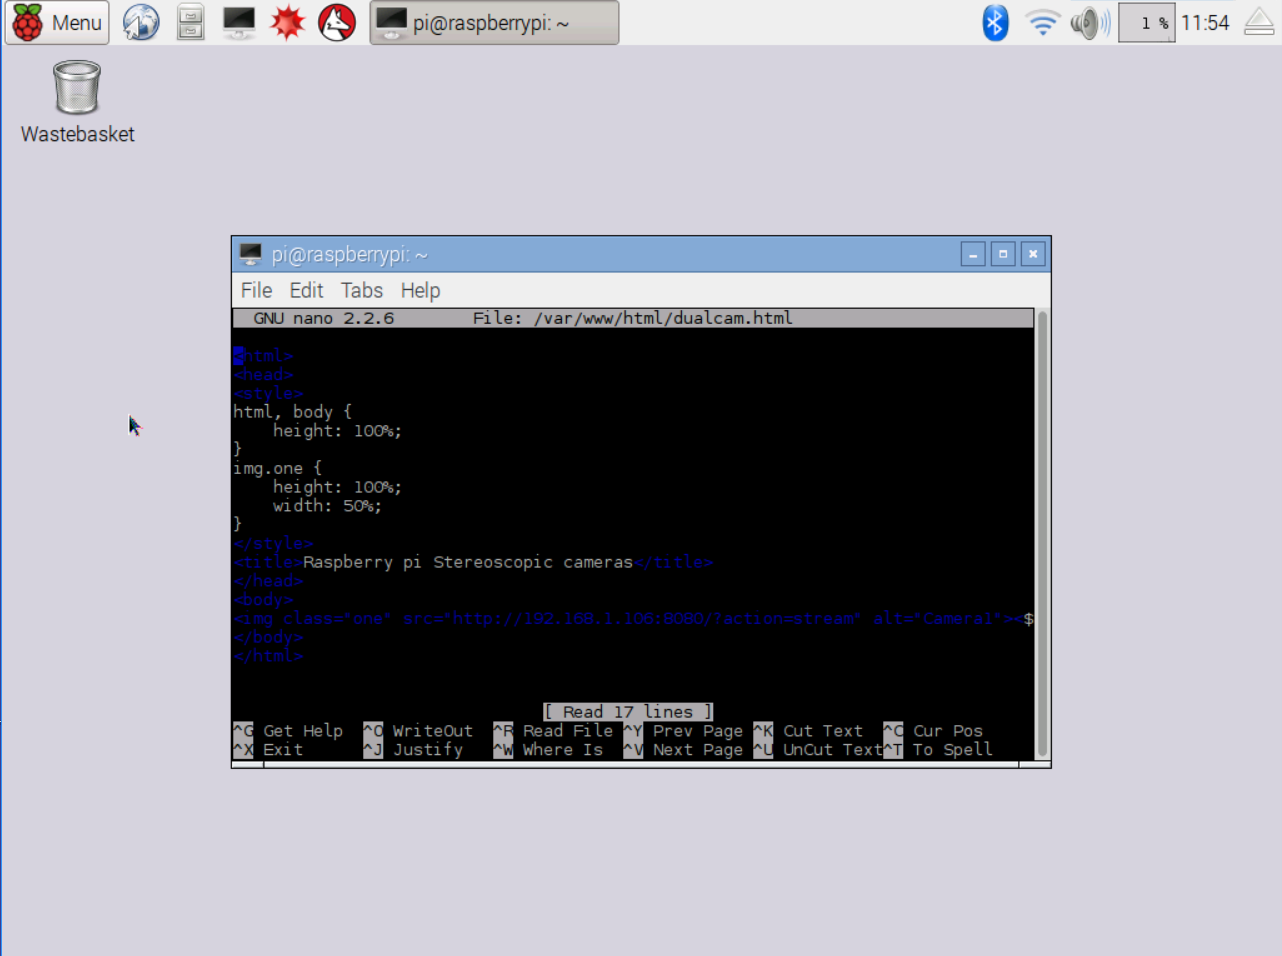
\includegraphics[width=\textwidth]{raspIDE.png}	
		\end{center}
		\legend{Fonte: Autor}
	\end{figure}

	\subsection{Particle IDE}\label{subsec-particleIDE}
	A Programação das placas Photon se deu pelo uso da Particle IDE, ambiente próprio para a programação das mesmas e que pode ser acessado através de um browser, sendo a tradução e envio do código às placas feito via nuvem própria.
			\begin{figure}[h!]
		\caption{\label{fig_particleIDE} Particle IDE  }
		\begin{center}
			\includegraphics[width=\textwidth]{ParticleIDE.png}	
		\end{center}
		\legend{Fonte: Autor}
	\end{figure}
	
	